\documentclass[12pt, fleqn]{scrartcl}

\usepackage[singlecolumn, german]{fnordstyle}
\usepackage{hyperref}
\usepackage{graphicx}
\usepackage{picins}
\usepackage{wrapfig}
\usepackage{verbatim}
\usepackage{tabularx}
\usepackage{csquotes}
\usepackage[style=mla, backend=biber]{biblatex}
\bibliography{oparl}
%\typearea{11}

\setlength{\abovecaptionskip}{-1em}
\setlength{\belowcaptionskip}{1em}
\let\oldnewcaption\newcaption
\renewcommand{\newcaption}[1]{
    \vspace{-1em}
    \oldnewcaption{#1}
    \vspace{1em}
}

\setcounter{tocdepth}{2}

\newcommand{\autocitenp}[2][]{\citeauthor{#2} \autocite*[#1]{#2}}

\hyphenation{mne-mon-ic}

\title{OParl-Validator-Protokoll}
%\subtitle{Flauschnotizen}
\author{Alex, Jo, Lucas, Ronald, Telofy}
\date{\today}

\begin{document}

\Maketitle

\section{Einführung}

\subsection{OParl}

Die Arbeit an OParl wurde begonnen, um einen einheitlichen Austausch von Parlamentsdaten zwischen Ratsinformationssystemen und Bürgerinformationssystemen zu ermöglichen, sowie auch, um Außenstehenden einen standardisierten Zugriff auf die verschiedenen genannten Systeme zu gewähren. Initiativen wie Offenes Köln, Frankfurt Gestalten und die Parlamentwatch e.\,V. haben bereits in begrenztem Rahmen aufgezeigt, welche Möglichkeiten in parlamentarischer Transparenz liegen, aber diese Lösungen sind noch stark dadurch eingeschränkt, dass sie zum Beispiel auf Screen Scraping von einem speziellen Ratsinformationssystem (RIS) basieren. OParl kann ihre Arbeit einfacher und universeller machen.

Die OParl-Initiative, geleitet von Jens Klessmann (Fraunhofer FOKUS), Marian Steinbach (Offenes Köln), Marianne Wulff (VITAKO) und Christine Siegfried (VITAKO), hat daher Kooperationen mit diversen RIS-Herstellern und transparenznahen Projekten geknüpft, und die Arbeit an dem gleichnamigen Kommunikationsstandard begonnen.

\subsection{Status}

Nachdem die Veröffentlichung von OParl schon von Anfang auf Ende Juni verschoben werden musste, stellte sich heraus, dass die geplante Verwendung von JSON-LD zu erheblichen Verzögerungen führen würde, und außerdem, wegen der geringen Verbreitung des Standards, auch Probleme für die RIS-Hersteller mit sich bringen würde. Die Entscheidung eine JSON-LD-Unterstützung auf eine spätere Version von OParl zu verschieben, rief interpersonelle Differenzen hervor, die in der Abspaltung eines konkurrierenden JSON-LD-Forks von OParl von einem der ehemaligen Entwickler kulminierte.

OParl wurde in Folge auf einen JSON-LD-losen Stand gebracht, doch auch die damit verbundenen Arbeiten sowie andere Korrekturen am Standard dauern weiter an.

\subsection{Validator}

Um den RIS-Herstellern und anderen interessierten Entwicklern eine einfache Möglichkeit an die Hand zu geben, zu testen, ob sie den Standard korrekt implementiert haben, war von Anbeginn an geplant, einen Validator für OParl zu entwickeln. Mit dem Start unseres Softwareprojektes bekam dieser Teilbereich unsere Verantwortlichkeit.

Der dynamische Zustand unseres Referenzstandards machte es notwendig, dass wir uns relativ beliebige aber möglichst günstige Commits der Spezifikation als Freezes herauspickten, um zunächst diese Versionen im Validator umzusetzen. Der lange Hiatus, der mit der JSON-LD-Debatte einherging, hielt somit den Validator für einige Zeit auf einem Stand der Spezifikation, der in Folge grundlegend umstrukturiert wurde. Dies bedeutete auch für uns einen Zeitverlust.

Da nunmehr immer noch keine 1.0-Version von OParl verabschiedet wurde, richten wir uns weiterhin nach einem solchen selbstgewählten Freeze (200606f).

\section{Organisation}
\section{Features}
\section{Demo}
\section{Architektur}

\begin{wrapfigure}{R}{0.5\textwidth}
  \begin{center}
    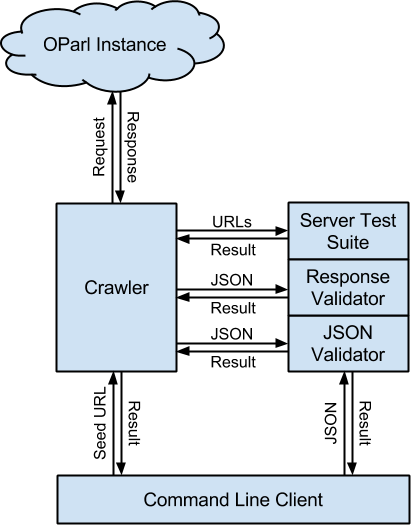
\includegraphics[width=.5\textwidth]{architecture.final.png}
  \end{center}
  \caption{Architektur}
\end{wrapfigure}

\subsection{Idee}

Die Grundidee hinter der Architektur unseres Projektes basiert auf dem Mantra, dass, wenn man ein Command-Line-Tool entwickeln möchte, man erst eine Library entwickeln soll, welche die eigentliche Arbeit verrichtet, und dann ein Command-Line-Tool als Frontend für sie schreiben soll.

Das ist eine nützliche Vorgehensweise, da sie alle Vorteile von Command-Line-Tools beibehält, während sie es Entwicklern ermöglicht, von der Flexibilität der eigentlichen Library zu profitieren. Git, zum Beispiel, basiert auf diesem Architekturprinzip.

In unserem Fall ist es so, dass es von Anfang an unser Anspruch war, beides, eine Library und ein Command-Line-Tool, zu entwickeln. Letzteres ist im selben Projekt aufgehoben, die Library aber kann auch mit anderen Frontends verwendet werden.

Die Validator-Library sollte zudem sowohl die Fähigkeit mitbringen, JSON-Daten direkt von der Command Line zu validieren, als auch die Standardfunktionalität, URLs eines OParl-Systems zu validieren. Zu diesem Zweck hat der Command-Line-Client zwei Code-Pfade, von denen einer den Validator direkt aufruft, während der zweite eine URL an einen Crawler als Seed übergibt.

\subsection{JSON-Validator}

Der Validator durchschreitet in seiner Tätigkeit verschiedene Phasen, zum Teil notwendiger Weise, und zum Teil, um bessere Fehlermeldungen ausgeben zu können. Hierbei mussten wir stets die Abwägung treffen, zu welchem Maße wir Leanness dem Komfort zu opfern bereit sind, den wir erwarten, die Benutzer° wertschätzen werden.

Zunächst wird das JSON selbst auf Fehler überprüft. Solche würden eine Weiterverarbeitung verhindern. Dann testet der Validator, ob ein gültiger Typ im Objekt spezifiziert ist. Ist das nicht der Fall, so können wir nicht schließen, welchem Format das Objekt folgen soll, und eine weitere Validierung ist auch ausgeschlossen.

Nach erfolgreichen Passierens dieser Phasen des Tests, kommt das JSON-Schema zum Einsatz, in das wir die Spezifikation übersetzt haben. Dieses Schema bildet das Herzstück des Validators, und ist versioniert, um mögliche zukünftige Versionen des Standards parallel unterstützen zu können. Alle Bestandteile des Schemas, die sich als JSON-Schema ausdrücken lassen, sind in diesen Dateien kodifiziert.

Letztlich gibt es noch einige Teile des Standards, die sich nicht im JSON-Schema abbilden lassen. Diese sind als Python-Funktionen implementiert und, mittels proprietärer Erweiterungen, im Schema referenziert.

\subsection{Response-Validator}

Neben dieser Kette an Validierungsschritten, gib es außerdem ein Validierungssystem für HTTP-Responses. Der Standard macht auch Vorschriften über die Headers, die ein Server ausliefern soll. Wenn der Validator also verwendet wird, um Antworten eines OParl-Servers zu validieren, so stellt dieser Teil des Systems sicher, dass sie Standardkonform sind.

\subsection{Server-Tests}

Es gibt eine Reihe weiterer Features von OParl, die es erfordern, dezidierte Requests zu senden, die zur Validierung der JSON-Objekte redundant wären. Unsere Test-Suite bedient sich an einer Liste von validen URLs von Crawler (der im Folgenden näher erläutert werden wird), und benutzt diese, um generische Eigenschaften und Fähigkeiten des Servers einer Prüfung zu unterziehen.

\subsection{Crawler}

% Outtake: Wenn das JSON-Schema das Herzstück unseres Validators ist, dann ist der Crawler Haut und Brustbehaarung.

Wenn das JSON-Schema das Herzstück unseres Validators ist, dann ist der Crawler seine Extremitäten und sein Schweif. Der Crawler folgt der üblichen Architektur, die aus einem Fetching-Modul, einem Link-Extractor und einem Hashtable als Speicher für bereits besuchte URLs besteht. Da er die geladenen JSON-Objekte \emph{just in time} validiert, müssen sie nach Abschluss der Validierung nicht länger vorgehalten werden. Gespeichert werden lediglich die URLs, wobei strenggenommen auch die URLs von validen und fehlerhaften Objekten unterschieden werden.

Die erste URL, die gespeichert wird, ist die Seed-URL, die man zum Beispiel via des Command-Line-Interfaces übergibt. Von dieser URL ausgehend, führt der Crawler eine gefilterte Breitensuche über dem OParl-Graphen durch, wobei die Filterkriterien, insbesondere die Typen-Whitelist, vom Nutzer° vorgegeben werden können.

Den Schweif des Crawlers bildet ein Aufruf der obengenannten Server-Tests mit den gesammelten validen URLs.

\section{Close-Out-Plan}

%\newpage

\phantomsection
\addcontentsline{toc}{section}{References}
\setlength\bibitemsep{0pt}
\printbibliography

\end{document}

Count
    
    grep -vE '^[\\ %}]' protocol.tex | wc
